\chapter{DESENVOLVIMENTO}

Neste capítulo são descritas as especificações formais da estrutura proposta e os ambientes, técnicas e ferramentas utilizadas para orientar como fazer a parte prática do projeto. 

\section{ESPECIFICAÇÕES FORMAIS}
São descritos os requisitos funcionais e não funcionais buscados no desenvolvimento da aplicação, além das especificações do projeto por meio de diagrama de \textit{deployment}, diagramas de classe, diagrama de sequência e diagrama de atividades.

\subsection{Descrição da Aplicação}
A aplicação proposta neste trabalho servirá apenas como exemplo para o objetivo principal que é o balanceamento de carga. A aplicação consiste em um controle de finanças pessoais, com a possibilidade de registrar proventos e despesas. Para o balanceamento de carga será preparada uma estrutura utilizando \textit{containers}, separando em três camadas: persistência de dados, regra de negócio e interface visual.

\subsection{Requisitos}
Segundo \cite{Pfleeger}, os requisitos são uma característica de um projeto, uma propriedade ou um comportamento do sistema, também pode ser a descrição de algo que o sistema é capaz de efetuar ou realizar. Portanto, cada requisito, por mais abstrato que seja,
pode ser uma condição ou capacidade do software para alcançar determinado objetivo. Nas próximas subseções são apresentados separadamente os requisitos funcionais e não
funcionais.

\subsubsection{Requisitos Funcionais}
Os requisitos funcionais definem as funções e o comportamento que o sistema deve oferecer ao usuário final \cite{Pressman}. Assim sendo, a Tabela \ref{Req-Func} demonstra todos os requisitos funcionais levantados:

\begin{table}[h]
	\caption{Requisitos Funcionais}
	\label{Req-Func}
	\begin{tabular}{|l|}
		\hline
		\textbf{REQUISITOS FUNCIONAIS} \\ \hline
		RF0: O sistema deve manter etiquetas \\ \hline
		RF1: O sistema deve manter transações \\ \hline
		RF2: O sistema deve manter períodos \\ \hline
		RF3: O sistema deve exibir o valor total de transações do período dividido entre proventos e despesas \\
		\hline
		RF4: O sistema deve exibir o valor total das transações de cada etiqueta do período \\ \hline
		RF5: O sistema deve exibir com base nas transações o valor que há na carteira \\ \hline
		RF6: Transações com data futura não devem afetar o valor da carteira \\ \hline
	\end{tabular}
\end{table}

\subsubsection{Requisitos Não Funcionais}
Segundo o autor \cite{Pfleeger}, um requisito do tipo não funcional (RNF) corresponde aos requisitos relacionados ao uso da aplicação em termos de exibição, desempenho, impressão, notificação, teste ou validação. RNF são os requisitos que definem características da aplicação relacionadas a confiabilidade, desempenho, usabilidade, entre outras. Em suma, pode ser definido em “como” o sistema vai fazer. A Tabela \ref{Req-Nao-Func} apresenta os Requisitos não funcionais do sistema.

\begin{table}[!h]
	\caption{Requisitos Não Funcionais}
	\label{Req-Nao-Func}
	\begin{tabular}{|l|}
		\hline
		\textbf{REQUISITOS NÃO FUNCIONAIS} \\ \hline
		RNF0: O sistema deve estar no ar 24 horas por dia \\ \hline
		RNF1: O sistema deve separar regras de negócio e persistência em \textit{containers} diferentes \\ \hline
		RNF2: O sistema deve aplicar balanceamento de carga \\ \hline
		RNF3: O sistema deve desenvolver as regras de negócio com a linguagem Java na versão 8\\ \hline
		RNF4: O sistema deve utilizar banco de dados PostgreSQL \\ \hline
		RNF5: O sistema deve utilizar \textit{containers} Docker \\ \hline
		RNF6: O sistema deve utilizar CORBA como \textit{middleware} \\ \hline
	\end{tabular}
\end{table}

\subsection{Especificações}
Nesta seção são apresentados os diagrama de \textit{deployment}, classe e de sequência, elaborados sob a Linguagem de Modelagem Unificada (\textit{Unified Modeling Language}, UML), para especificação do sistema proposto.

\subsubsection{Diagrama de \textit{Deployment}}
No diagrama de \textit{deployment} apresentado na Figura \ref{Diagrama-Deployment} são demonstrados os componentes presentes na estrutura a ser desenvolvida, cada componente terá uma função e realizarão comunicação entre si utilizando o \textit{middleware} CORBA.

A estrutura é separada em três partes: \textit{Application, Controller Server e Database Server}. A primeira é responsável por realizar a interação com o usuário, apresentar a interface visual e executar as requisições solicitadas pelo usuário. O \textit{Controller Server} recebe as solicitações do usuário e faz o manuseio dos dados, validando as informações e aplicando as regras de negócio necessárias. Por fim, temos o \textit{Database Server} que tem como função exclusiva a persistência de dados, ele salva e lê o que for solicitado pelo \textit{Controller}.

\begin{figure}[htb]
	\caption{Diagrama de \textit{Deployment}}
	{\parbox{6cm}{
			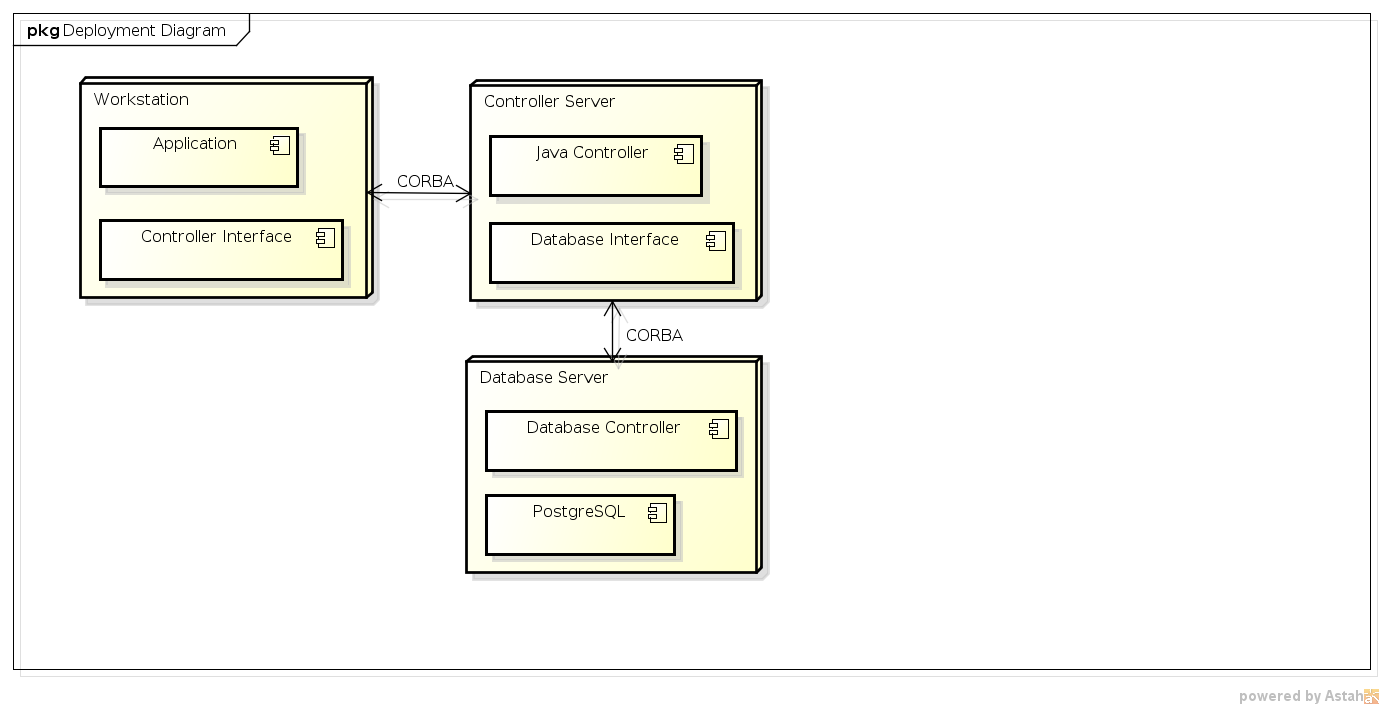
\includegraphics[width=14cm]{images/DeploymentDiagram.png}
			\label{Diagrama-Deployment}
			\fonte{Acervo do autor}
	}}
\end{figure}

\subsubsection{Diagrama de Classe}
As classes que compõem o sistema, bem como as relações entre cada classe, são apresentadas
na Figura \ref{Diagrama-Classe} e servem também para a modelagem do \textit{middleware}.

As classes \textit{Transaction, Tag} e \textit{Period} servem para armazenamento e transição de informações, não apresentam nenhum método. O manuseio dos dados é executado pelas classes \textit{TagController} e \textit{PeriodController}, que por sua vez não necessitam de atributos.

\begin{figure}[!htb]
	\caption{Diagrama de Classe}
	{\parbox{6cm}{
			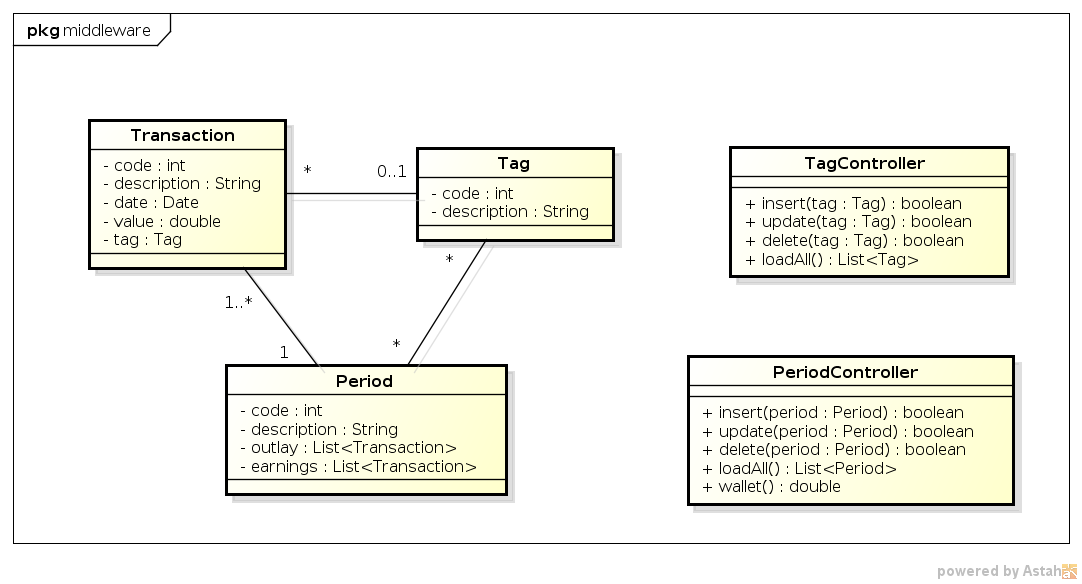
\includegraphics[width=10cm]{images/ClassDiagram.png}
			\label{Diagrama-Classe}
			\fonte{Acervo do autor}
	}}
\end{figure}

\subsubsection{Diagramas de Sequência}
Os diagramas de sequência das figuras \ref{SeqTag}, \ref{SeqPeriod} e \ref{SeqTransaction} apresentam os fluxos básicos da aplicação. A partir deles é possível conhecer as principais funções do sistema.

O processo de criação de \textit{Tag} está apresentado na Figura \ref{SeqTag} e consiste na criação por parte do usuário de uma nova instância do modelo \textit{Tag}, preenchimento dos seus dados e envio ao controlador para validação, em caso positivo é solicitado ao servidor de persistência para que a nova \textit{Tag} seja salva e uma mensagem de sucesso é retornada ao usuário.

\begin{figure}[!htb]
	\caption{Diagrama de Sequência de adição de \textit{tag}}
	{\parbox{6cm}{
			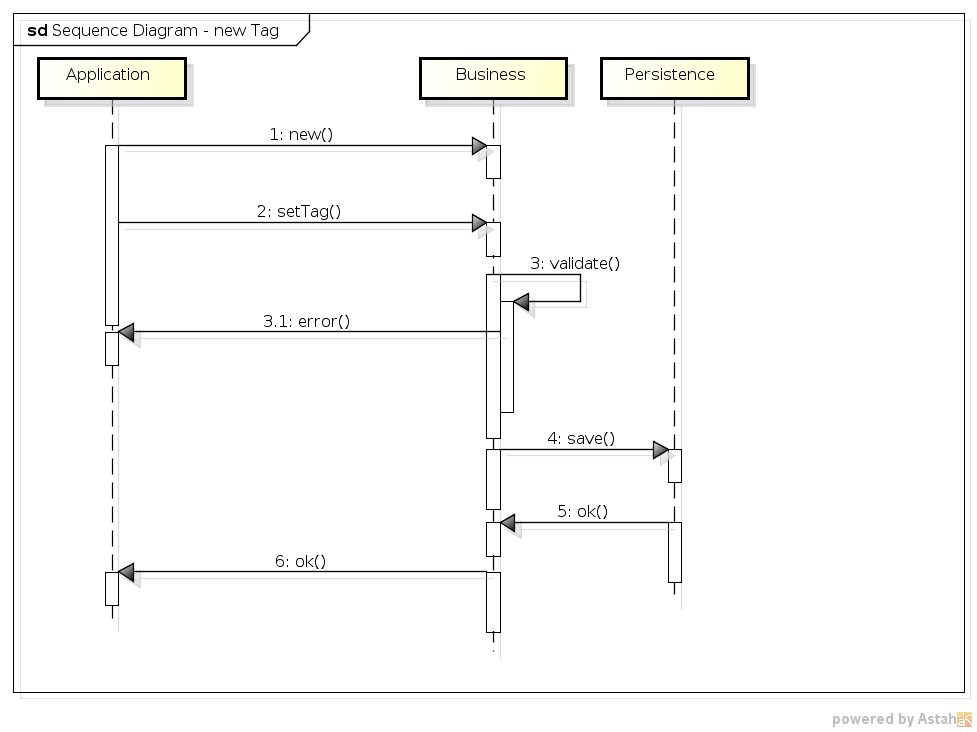
\includegraphics[width=10cm]{images/SequenceDiagramNewTag.png}
			\label{SeqTag}
			\fonte{Acervo do autor}
	}}
\end{figure}

A Figura \ref{SeqPeriod} apresenta a criação de um novo período no sistema, este receberá uma descrição e abrirá uma nova lista de transações. O servidor de controle validará as informações e enviará a persistência para que o novo período seja salvo.

\begin{figure}[!htb]
	\caption{Diagrama de Sequência de adição de Período}
	{\parbox{6cm}{
			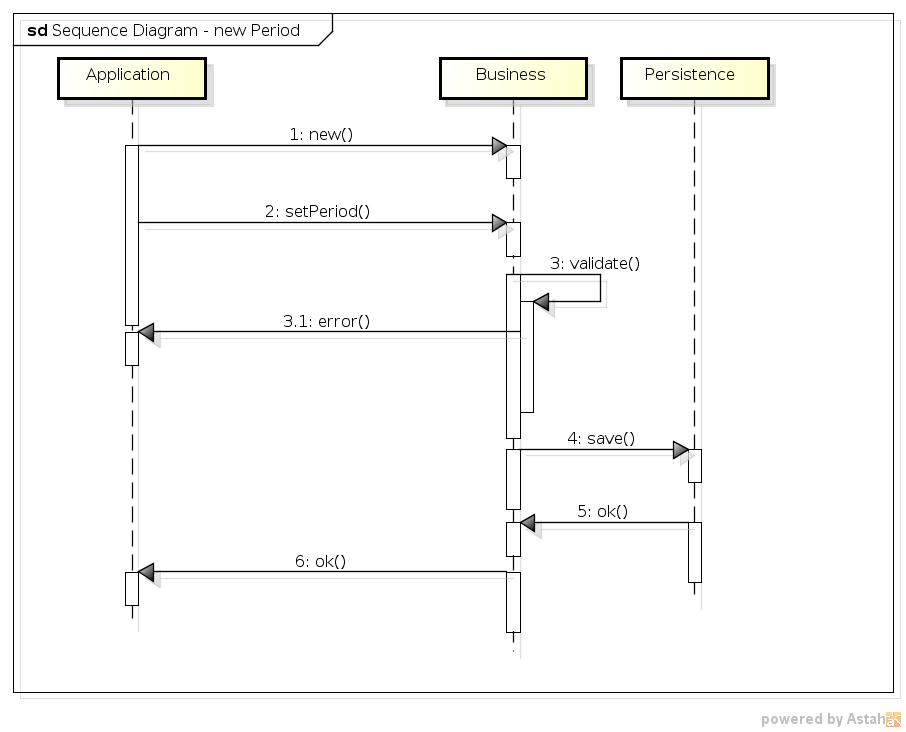
\includegraphics[width=10cm]{images/SequenceDiagramNewPeriod.png}
			\label{SeqPeriod}
			\fonte{Acervo do autor}
	}}
\end{figure}

Após ter um período criado é possível adicionar transações de ganhos ou despesas a ele. Uma nova transação deverá ter uma descrição, valor e data, podendo ser atribuído uma \textit{tag}. Ao finalizar o cadastro a aplicação repassa a solicitação para o servidor de controle, que valida as informações e envia para persistência. Sempre que o processo ocorrer corretamente a lista de transações é atualizada, bem como o valor na carteira. Este fluxo está presente da Figura \ref{SeqTransaction}.

\begin{figure}[!htb]
	\caption{Diagrama de Sequência de adição de transação}
	{\parbox{6cm}{
			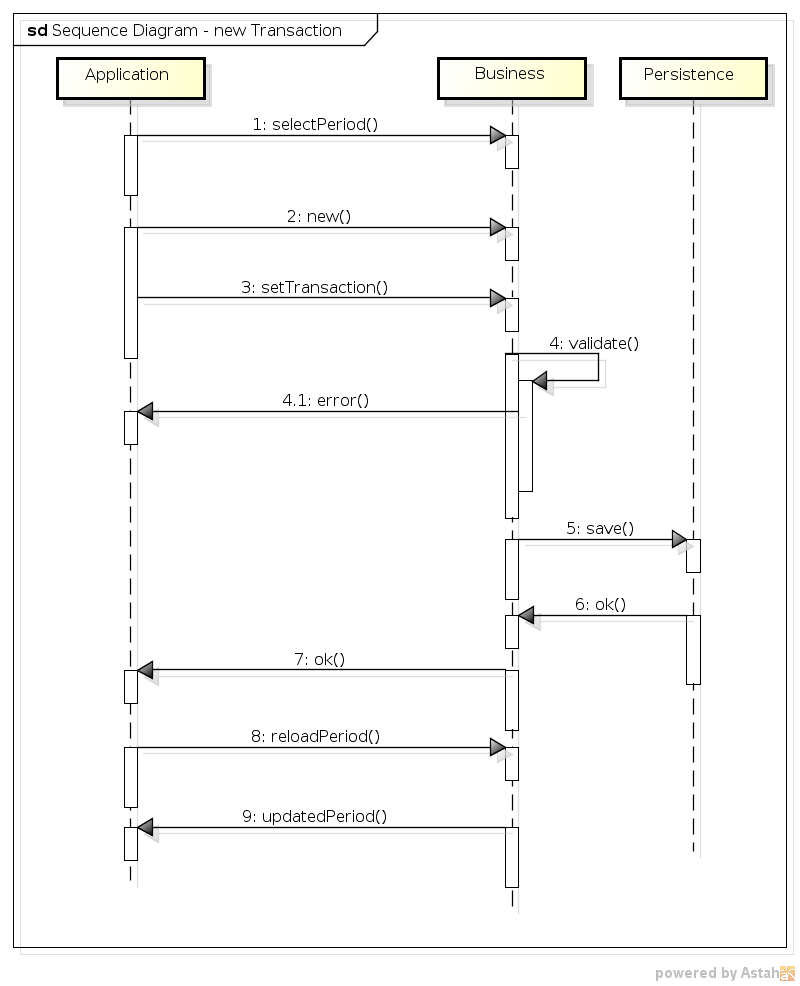
\includegraphics[width=10cm]{images/SequenceDiagramNewTransaction.png}
			\label{SeqTransaction}
			\fonte{Acervo do autor}
	}}
\end{figure}

\section{Exposição do Tema ou Matéria}